\subsection{\textit{Pygov-br}}

\textit{Pygov-br} é uma biblioteca \textit{python} desenvolvida no contexto desse trabalho cujo objetivo é centralizar o consumo de \textit{APIs} e \textit{webservices} governamentais brasileiros. Além dos dados, a biblioteca também irá fornecer um conjunto de \textit{plugins} para os principais \textit{frameworks} para desenvovimento \textit{web}, para facilitar a utilização dos dados abertos, bem como o cruzamento de dados provenientes de diferentes órgãos governamentais.

Atualmente, a biblioteca oferece suporte somente ao \textit{webservice} da Câmara dos Deputados, tanto para o consumo dos dados quanto para o uso em aplicações \textit{Django}, já que para o desenvolvimento do presente trabalho apenas esses dados seriam utilizados.

A estrutura para o consumo dos \textit{webservices} não é fixa, pois cada \textit{webservice} possui suas características. A implementação para consumir os dados da Câmara dos Deputados segue a estrutura do \textit{webservice} (figura \ref{estrutua_camara_deputados}), com alterações em alguns \textit{endpoints}, conforme mostra a tabela \ref{alteracoes-estrutura-webservice}. Além disso, todos o código implementado foi escrito em inglês, apesar dos dados estarem em português.

\begin{figure}[h]
    \centering
    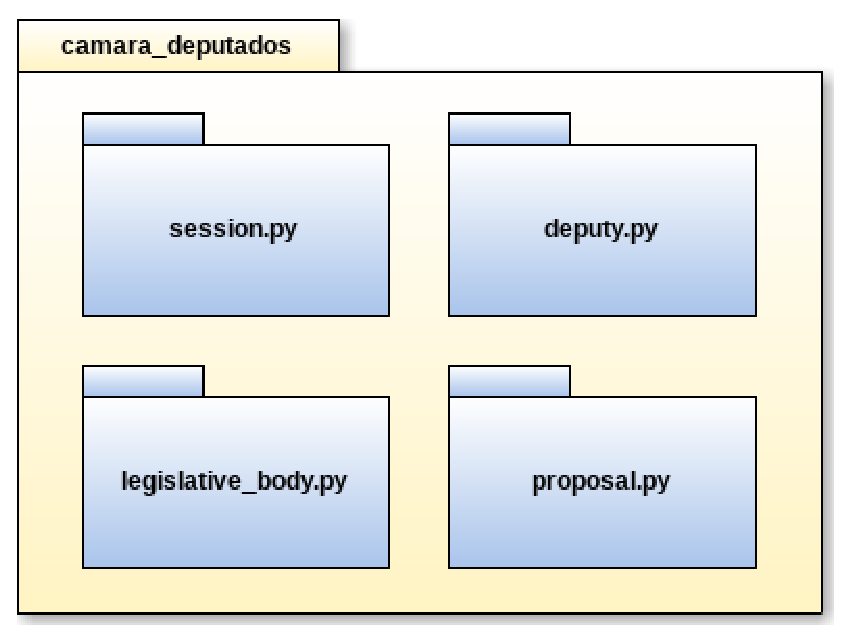
\includegraphics[scale=0.5]{figuras/camara_deputados.eps}
    \caption{Estrutura do módulo de consumo de dados da Câmara dos Deputados}
    \label{estrutua_camara_deputados}
\end{figure}

\begin{table}[h]
\centering
\begin{tabular}{|l|c|c|}
\hline
\multicolumn{1}{|c|}{\textit{\textbf{Endpoint}}} & \multicolumn{1}{c|}{\textbf{Módulo Final}} & \multicolumn{1}{c|}{\textbf{Estrutura do \textit{Webservice}}} \\ \hline
ListarPresencasParlamentar & deputy.py & SessaoReuniao \\ \hline
ObterAndamento & proposal.py & Orgao \\ \hline
ObterEmendasSubstitutivoRedacaoFinal & proposal.py & Orgao \\ \hline
ObterIntegraComissoesRelator & proposal.py & Orgao \\ \hline
\end{tabular}
\caption{Alterações na Estrutura do \textit{Webservice} da Câmara dos Deputados}
\label{alteracoes-estrutura-webservice}
\end{table}

Como dito anteriormente, a \textit{pygov-br} também possui módulos para utilização em conjunto com os \textit{frameworks} de desenvolvimento \textit{web} mais utilizados na comunidade. Porém, como a solução \textit{web} desenvolvida nesse trabalho utilizará o \textit{framework Django}, a atual implementação da \textit{pygov-br} possui suporte somente a esse \textit{framework}.

O módulo \textbf{django\_apps} contém os \textit{plugins} para utilização em projetos \textit{Django}, o que implica na uso da arquitetura \textit{MVT} (\textit{Model View Template}). Similar ao \textit{MVC}, no \textit{MVT} o ciclo começa por uma ação do usuário, a View notifica a Model, para que seu estado seja atualizado, a Model efetua as modificações necessárias e alerta as suas dependências que foi alterada, assim a Template consulta o novo estado da Model, e atualiza a sua visualização.

Entretanto, os \textit{apps Django} da \textit{pygov-br} possuem apenas as \textit{models}, já que o objetivo é somente facilitar a permanência das informações obtidas dos \textit{webservices} governamentais em um banco de dados. No caso da Câmara dos Deputados, os dados utilizados nesse trabalho ficam disponíveis seguindo o modelo entidade-relacionamento na figura \ref{modelo-eer}. Podemos notar que todas as colunas de todas as tabelas se encontram em em inglês, por motivos de padronização do código.


\begin{figure}[h]
    \centering
    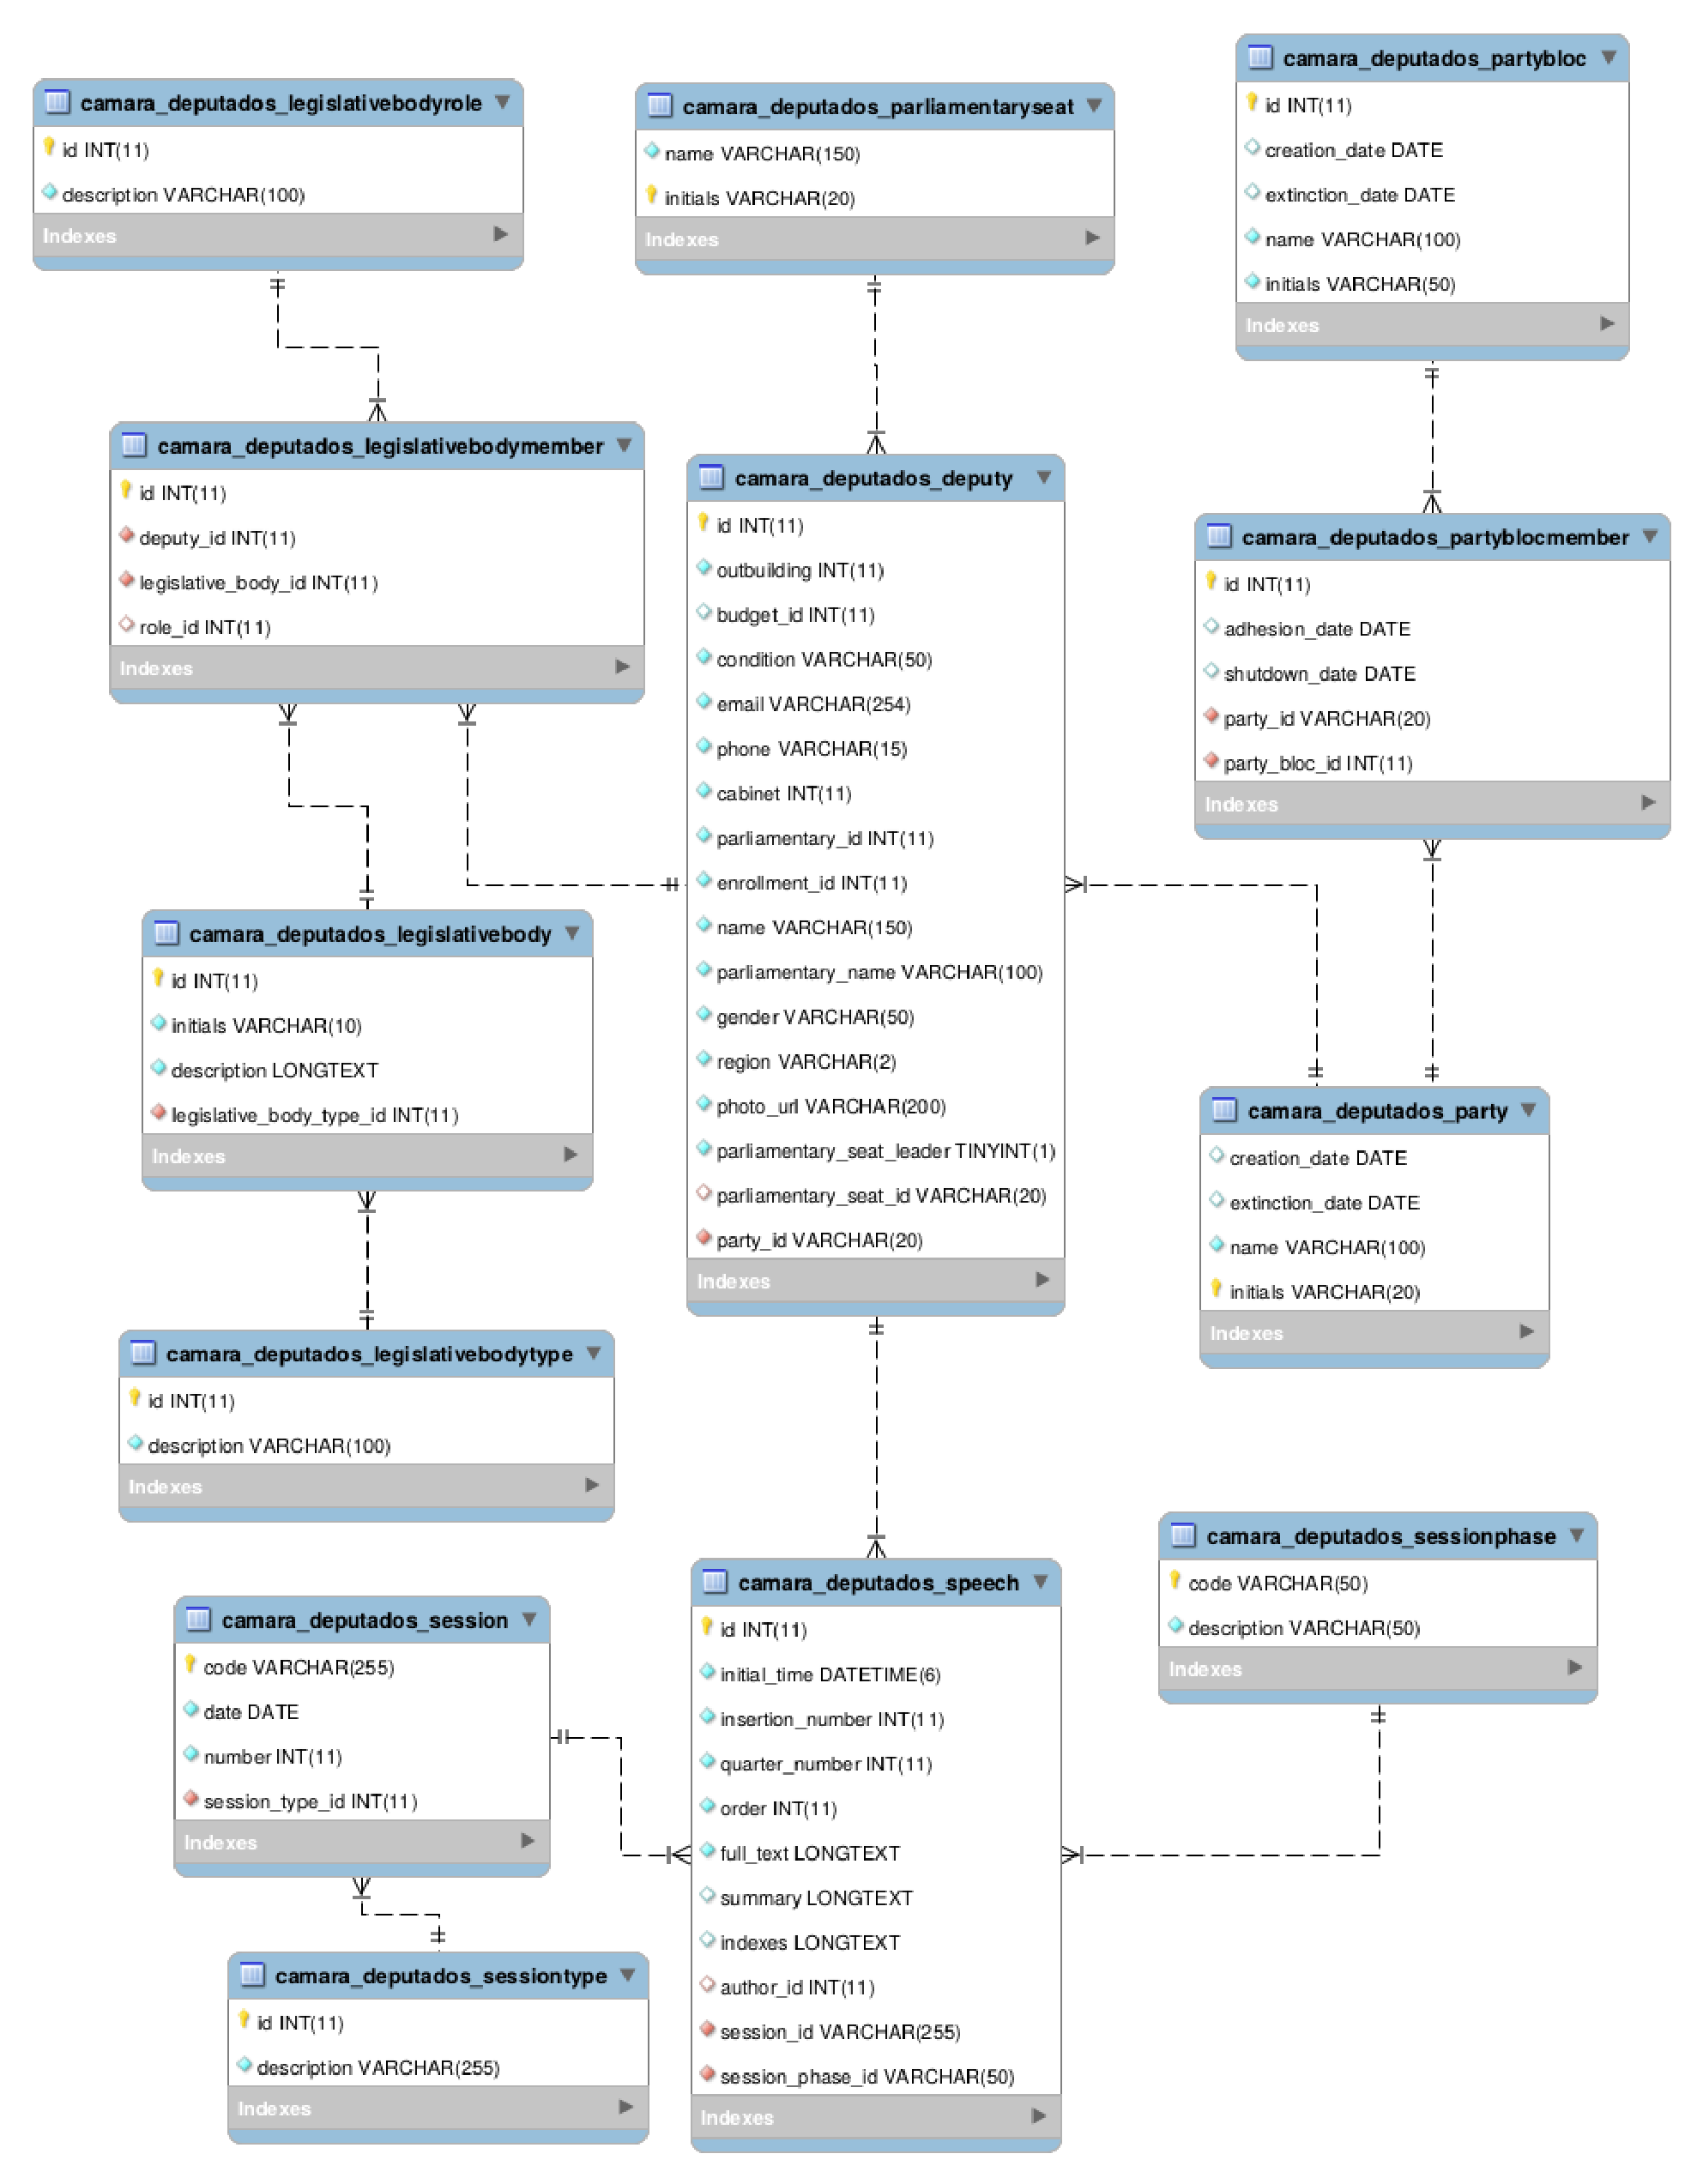
\includegraphics[scale=0.5]{figuras/pygov-eer.eps}
    \caption{Modelo entidade-relacionamento do banco de dados utilizado}
    \label{modelo-eer}
\end{figure}
